\subsection{Mutierende globale Problemmenge}
\begin{figure}[h]
  \centering
  \includegraphics[width=0.77\textwidth]{images/E_G_abab_solved.pdf}
  \caption[ABAB Problem - Globale, mutierende Problemmenge]{ABAB Problem - Globale, mutierende Problemmenge}
  \label{fig:e_g_abab}
\end{figure}
Die untersuchten evolutionären Algorithmen mit einer globalen mutierenden Problemmenge haben im Gegensatz zum Ansatz mit den Festen globalen Problemmengen ein abweichendes Konvergenzverhalten im Bezug auf die Grösse der Problemmenge an den Tag gelegt.

Die Eingabeparameter für die Abbildung \ref{fig:e_g_abab} waren:
\begin{itemize}
	\item Problemmengengrösse: 50, 100, 150, 200, 250
	\item Populationsgrösse: 50, 100, 150, 200, 250
\end{itemize}

In Abbildung \ref{fig:e_g_abab} ist ersichtlich wie sich ein \flqq teppenförmiges\frqq Muster abzeichnet. Daraus erschliesst sich die These, dass der Algorithmus unabhängig von der Problemmengengrösse eigentlich immer gleich oft konvergiert. Um diese These zu überprüfen wurde auch mit diesem Algorithmus ein Test bei konstanter Populationsgrösse durchgeführt. Als Problem der Wahl wurde hier aus Gründen der Vergleichbarkeit wieder das durch fünf Teilbar Problem gewählt.
\begin{figure}[H]
  \centering
  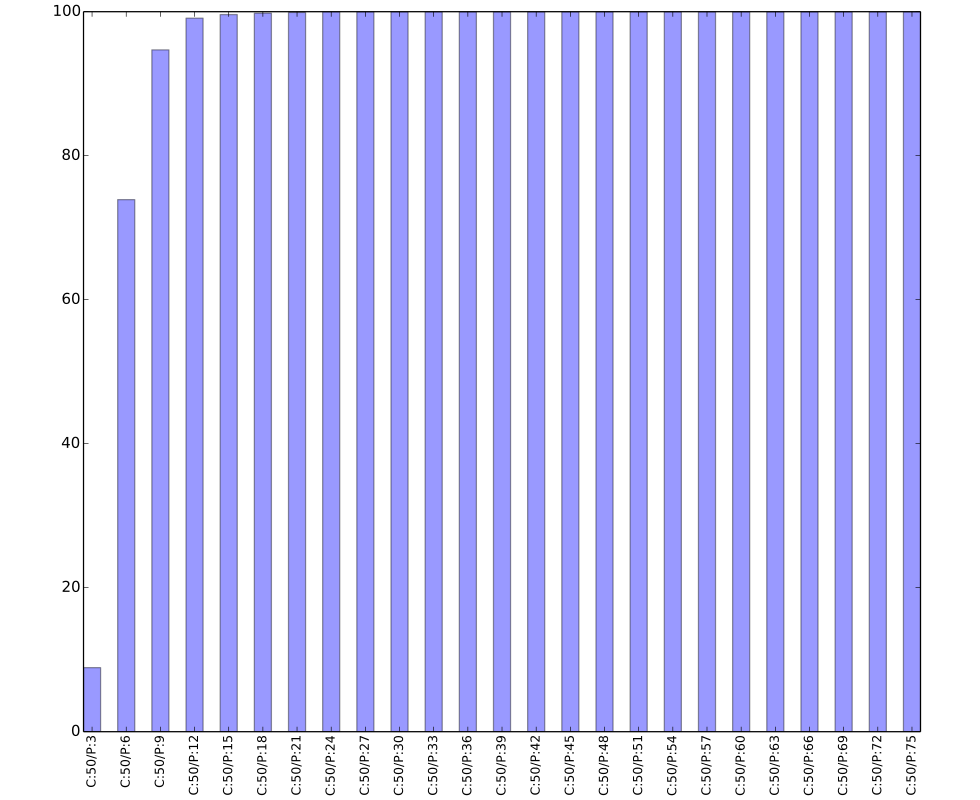
\includegraphics[width=0.77\textwidth]{images/E_G_PS_div5PS_solved.pdf}
  \caption[\Gls{e_g_alg} - Skalierung mit Problemmengengrösse]{\Gls{e_g_alg} - Skalierung mit Problemmengengrösse}
  \label{fig:e_g_ps_div5}
\end{figure}
Die Eingabeparameter für die Abbildung \ref{fig:e_g_ps_div5} waren:
\begin{itemize}
	\item Problemmengengrösse: 3, 6, 9, 12, ..., 72, 75
	\item Populationsgrösse: 50
\end{itemize}

Bei diesem Versuch (Abbildung \ref{fig:e_g_ps_div5}) sieht man, dass auch dieser Algorithmus mit sehr kleinen Problemmengen ($3$ oder $6$ Probleme) mühe hat. Jedoch konvergiert er bereits ab circa 10 Problemen in jedem Fall. Das heisst, sobald eine kritische Problemmengengrösse erreicht wurde, hat ein weiteres erhöhen dieser keinen Einfluss mehr auf das Ergebnis.

Das bedeutet, dass diese Art von evolutionären Algorithmen primär mit der Populationsgrösse skalieren. Welches die Optimale Problemmengengrösse für ein konkretes Problem ist, muss individuell geprüft werden. Für unser Problem der durch fünf teilbaren Binärzahlen konvergiert der Algorithmus zum Beispiel bereits ab 20 Problemen sehr zuverlässig.

Um zu prüfen wie das Konvergenzverhalten in Abhängigkeit der Populationsgrösse ist, wurde auch hierzu entsprechende Daten gesammelt.
\begin{figure}[H]
  \centering
  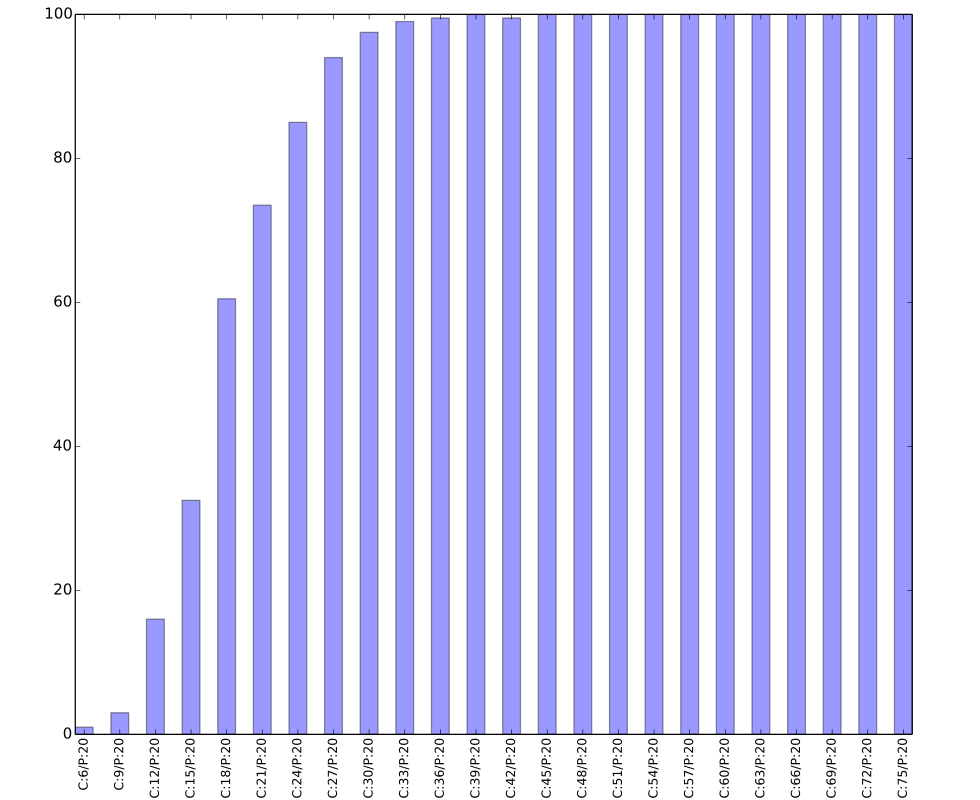
\includegraphics[width=0.78\textwidth]{images/E_G_CS_div5CS_solved.pdf}
  \caption[\Gls{e_g_alg} - Skalierung mit Populationsgrösse]{\Gls{e_g_alg} - Skalierung mit Populationsgrösse}
  \label{fig:e_g_cs_div5}
\end{figure}
\clearpage
Die Eingabeparameter für die Abbildung \ref{fig:e_g_cs_div5} waren:
\begin{itemize}
	\item Problemmengengrösse: 20
	\item Populationsgrösse: 3, 6, 9, 12, ..., 72, 75
\end{itemize}

In dieser Abbildung sieht man erneut, dass eine zu kleine Population ein Problem ist. Der steile Anstieg der Konvergenzrate und das Abflachen (in diesem Fall sogar erreichen der 100\% Marke) ist vergleichbar mit dem Verhalten des Algorithmus mit konstanter Problemmenge.